\chapter{Appendix}
\section{Hardware}\label{hardware}
The training experiments were performed using a high-performance machine learning PC. It had 64 AMD Radian Cores, two Nvidia GeForce RTX 2080 with 11 GB of video memory each, 128 GB of RAM, 256 GB SSD and a 6TB HDD.

Also, a PC running Microsoft's Windows 10 with 8 Intel i9 processors, one Nvidia GeForce GTX 1080 Ti and 64 GB RAM were used to run the VBS3 simulations in order to generate the synthetic dataset. It was possible to run up to 8 parallel instances of VBS3 on the highest graphical settings without significantly slowing down the image generation.

\section{VBS3 Vehicle Dataset}\label{dataset-result}
The work performed during this thesis has resulted in a large meta-learning data set with high-quality images and a large set of labels for each image. This section will, in detail describe the dataset used in this thesis, which has been named the VBS3 Vehicle Dataset. It will outline all the information that is provided for each data-point how they have been used in this thesis and possible future applications.

\subsection{Images}
Each image is a 1280 x 768 RGB color image in PNG format.

\subsection{Vehicle Classes}
The VBS3 Vehicle Dataset contains a selection of vehicle models taken from the VBS3's internal list of vehicle models available in version 18.3.3.8. In total there exist 2381 unique models in this dataset. 

\subsection{Image Background}\label{settings}
In order to increase the variation in the data, the models are spawned into a range of pre-built environments. These five were selected due to them both being the most detailed and with the best-looking texture assets. Each image is therefore tagged with the name of the environment in which it was taken. These include: 

\begin{itemize}
    \item \textbf{Tropical}: A tropical environment covered mostly with forest and a large river.
    \item \textbf{Afghanistan}: A desert-like landscape.
    \item \textbf{USA}: A small American town surrounded by open fields.
    \item \textbf{Eastern European}: A coniferous forest with a small lake.
    \item \textbf{Iraq}: A large Middle Eastern city surrounded by open desert.
\end{itemize}

\subsection{Vehicle Data}\label{vehicle-data}
For each object in the image has a set of corresponding meta information: object bitmap, object bounding-box, object color scheme, and object rotation.

\textbf{Bitmap}: The bitmap is a binary 2D vector that segments the original image into two segments: the pixels which contain the object, and those who do not (see Figure \ref{bitmap}). The segmentation produced are pixel perfect except for some models where parts of the vehicle are consistently missing, due to them not being appropriately masked by the engine.

\begin{figure}[H]
\centering
\subcaptionbox{Original Image}
  {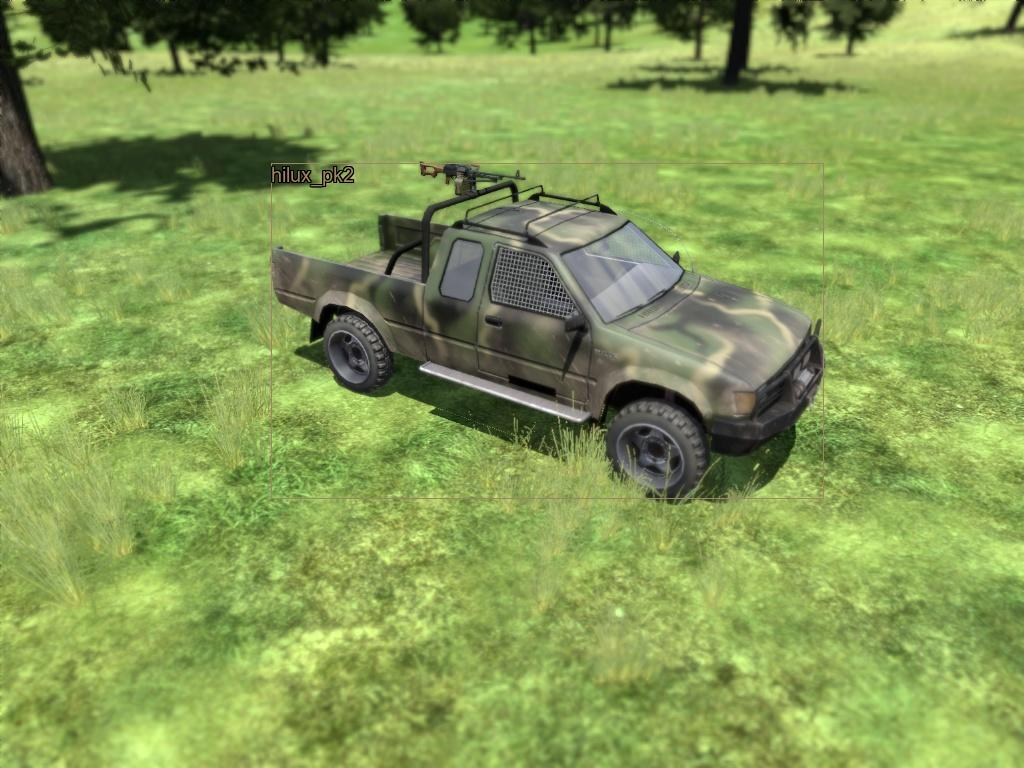
\includegraphics[height=4.4cm]{images/vbs3/bitmap/example3.jpg}}
\subcaptionbox{Bitmap}%
  {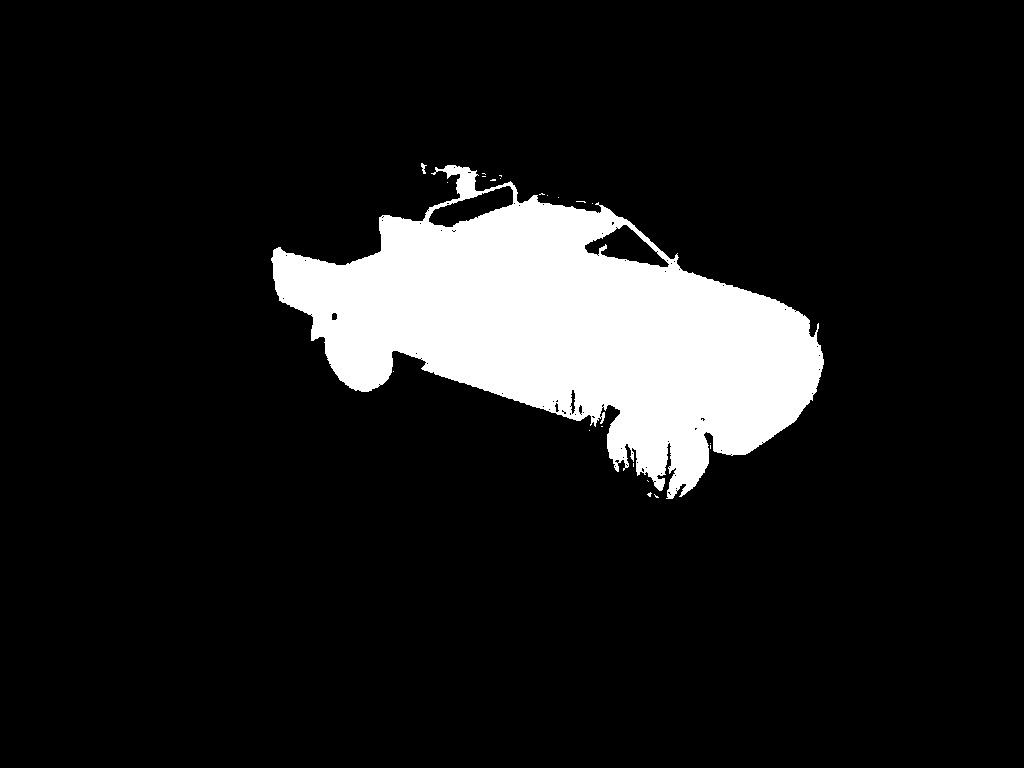
\includegraphics[height=4.4cm]{images/vbs3/bitmap/example3-bitmap.jpg}}
  \caption{}
\label{bitmap}
\end{figure}

\textbf{Bounding Box}: The bounding boxes consist of four values. The x and y pixel index of the leftmost lowest point of the box, and its width and height in the number of pixels.

\textbf{Rotation}: The rotation for each object is given as yaw, pitch, and bank. Although not utilized in this thesis, these values can be used in a myriad of ways. All the values are given in degrees. 

\begin{itemize}
    \item \textbf{Yaw} refers to the rotation around an axis drawn from the top to bottom. If all other rations are fixed a vehicle with a yaw of zero degrees will be facing the camera head-on, while a yaw of 90 will have the vehicle facing to the right of the image.

    \item \textbf{Pitch} refers to the rotation around an axis going from the left side to the right side of the vehicle. If all other rations are fixed a vehicle with a pitch of 0 will be facing straight forward, while a pitch of 90 degrees means that the vehicle will be looking straight up.

    \item \textbf{Bank} refers to the rotation along an axis going from the front to the back of the vehicle. If all other rations are fixed a bank of 90 degrees means that the object will be lying on its right side.
    
\end{itemize}

\textbf{Color Scheme}: Some of the models have been randomly assigned a set of colors in some subset of the pictures. Each color is sampled uniformly from the possible set RGB values, and alpha is uniformly sampled between 0.5 and 1.0. If a random color selection has been applied to a model in an image, this is saved as a list of 4-grams. Each 4-gram corresponds to the RGBA values of the reassigned texture. 

The degree to which the colors are randomized is reliant on what VBS3 supports, and the quality of the randomized models can vary. The data has been generated in such a way as to by randomly assigning a color to each texture in the model. As a result, the number of colors which are randomized per vehicle is dependent on the number of unique textures that make up the vehicle. As a result, some randomized vehicles are given a single uniform color, while others can consist of a large set of colors (see Figure \ref{color-scheme}).

\textbf{Weather}: Each image is provided with the weather setting, which was enabled when the photo was taken. The configuration is given as three values between zero and one. They correspond to the level of rain, level of fog, and level of overcast, with a higher value corresponding to more intense weather settings.

\textbf{Crepuscular Rays}: Each image is also provided with the scattering coefficients for the Crepuscular Rays/God Rays. The configuration is provided as three values between zero and thirty. They correspond to the relation between the three RGB channels, as well as how much the light should fracture when colliding with something.